\documentclass{standalone}
% preamble: usepackage, etc.
\begin{document}
	
\chapter{基于强化学习的路径规划算法}
在这一章我们将给出用于路径规划问题的强化学习算法的描述,包括了首先将路径规划这一图论问题转化到马尔科夫决策过程,这使得我们可以应用强化学习解决该问题。其次我们针对多个不同的场景设计了不同的算法,并给出这样设计的原因。\par
传统的路径规划算法对待该问题的形式为,在预处理阶段,首先在图上按照算法进行一定的计算和结果的存储,如存储两点间的最短路径距离,路径经过的节点等信息,也有部分较复杂的算法,对其做缩点等图上的优化操作等,第二步进入查询阶段,即根据用户给定的起点和终点,通过预处理得到的结果再给出最终的最短路径规划结果。这一建模方法并不是一个典型的强化学习建模方式,因此在应用到强化学习到该问题时,我们需要变换问题的形式为,在给定某个地图环境后,我们先经过一个强化学习算法学习过程,例如 Q-Leanring 方法,得到一个最优的策略函数和价值函数,这一步等同于传统算法的预处理阶段,第二步,对于查询,我们直接将学习到的策略部署到用户端。在任意时刻,给定当前的状态,给出选择后的行为,因此规划过程变成了在线过程,而非离线。同样如果需要达到离线规划的效果,我们需要该策略对应环境下的模拟环境,通过给定初始状态和模拟环境,得到完整的规划路径后返回结果给用户。具体的流程如图\ref{fig:system}所示。在我们的方法中,我们只关注相关算法的设计,对于一个完整的路径规划系统的设计不在我们的研究范畴。\par
\begin{figure}[H]
    \centering
    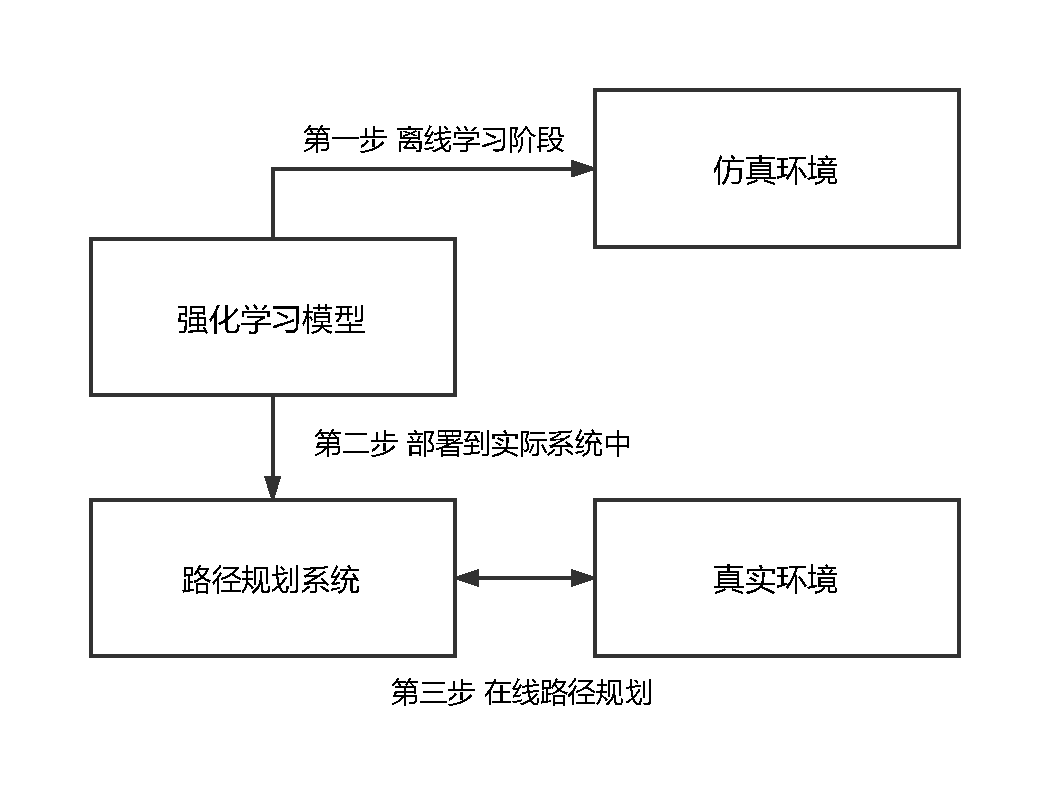
\includegraphics[width=9.0cm]{pic/system.pdf}
    \caption{基于强化学习的路径规划系统}
    \label{fig:system}
\end{figure}
在算法上,我们设计了一个端到端的系统,即模型的决策系统输入为环境的原始状态,输出也为环境的原始行为。端到端的设计具有以下几种优势,首先其使得我们的模型更易于优化,如果我们将模型拆分成多个子模块,那么对于每个模块我们需要单独设计其优化算法,这大大增加了算法的设计和调试难度。其次通过端到端的模型,更能现有的深度学习算法的能力,在早期的人工智能领域,因为限于当时的计算能力和数据量,比较流行的算法往往加入了大量的人类的先验,但随着计算能力的快速提高,大数据的出现,端到端的模型因此展现出了巨大的能力,在多个领域和问题获得了非常好的结果\citing{Mnih2013Playing, David2016Mastering}。因此在我们的算法中,我们也将采用端到端的设计。\par

\section{基于马尔科夫决策过程的算法形式表述}
在这一节,我们将路径规划问题表述为一个建立在离散时刻上的马尔科夫决策过程,给出其状态空间$S$,行为空间$A$,状态转移函数$P$,奖赏函数$R$等马尔科夫决策过程的几个基本元素的定义。然后针对不同的场景,我们提出了基于
Q-leanring 的算法。针对每个不同的场景,我们对算法做了相应的调整,并给出这样设计的思路和原因。\par
通过使用网格地图作为我们的环境,比较易于将智能体在任意一个状态下的行为选择规约到一个固定的状态集合上,如果不按照此建模方式,我们需要提出一个更灵活的对行为和状态建模的方式,而非端到端的方式,关于这一方向的讨论我们将在最后一章总结和未来方向中进行讨论。

\section{不同场景下算法设计方法}
在这一章,我们定义四个场景的对应马尔科夫决策过程的严格定义,同时给出相应的算法。第二,三,四个场景都部分的基于场景一,然后同时根据场景的特性,做了相应的更改。我们希望四个场景能尽可能多个共享相同的建模上的设计,这样使得算法设计能够具有更好的通用性使得其并不被完全限制于该场景下,以及更进一步的,提出一个单一的集合模型使得其能够同时解决多个场景下的规划问题。
\subsection{场景1:简单网格地图}
首先对于一个简单的$N \times M$大小的网格地图,由于在任意时刻,车辆可以在不超出地图边界的情况下向上下左右四个方向移动,同时不考虑任何对车辆的行驶限制。因此对该场景的状态定义为$s_t^{case1} = (x_t^{car}, y_t^{car}, x^{target}_t, y^{target}_t)$,其中 $x_t^{car}, x^{target}_t=0..N-1, y_t^{car}, y^{target}_t=0..M-1$, 其中$(x_t^{car}, y_t^{car})$表示车辆当前位置,$(x^{target}_t, y^{target}_t)$ 表示目标位置。其行为集合定义为$a_t^{case1} \in \{Up, Down, Left, Right\}$分别表示向上,下,左,右行驶。对于状态转移函数$P^{case1}{(s_{t+1}^{case1}|s_t^{case1}, a_t^{case1})}$的设计,我们限制车辆每个时刻只能移动一个单位的距离,同时不能超出边界,因此将状态转移表述为一个确定性过程,同时我们需要特殊判断是否车辆会超出地图边界,如果超出,维持原状态。定义公式如式\ref{case1P}。
    \begin{equation}
    \label{case1P}
    s_{t+1}^{case1} = \begin{cases}
    (x_t^{car}, y_t^{car}, x^{target}_t, y^{target}_t) &\mbox{if car will reach out of map}\\
    (x_t^{car} + 1, y_t^{car}, x^{target}_t, y^{target}_t) &\mbox{if $a_t$ is Right}\\
    (x_t^{car} - 1, y_t^{car}, x^{target}_t, y^{target}_t) &\mbox{if $a_t$ is Left}\\
    (x_t^{car}, y_t^{car} + 1, x^{target}_t, y^{target}_t) &\mbox{if $a_t$ is Up}\\
    (x_t^{car}, y_t^{car} - 1, x^{target}_t, y^{target}_t) &\mbox{if $a_t$ is Down}
    \end{cases}
\end{equation}
奖赏函数的设计是强化学习中一个核心的部分,特别是对于给定的场景本身不存在一个原有的奖赏产生机制时,我们需要手动设置和调整奖赏函数的设计,作为唯一指导智能体进行学习的信号,我们需要将学习目标或评价机制通过奖赏函数体现出来。而设计奖赏函数需要遵循以下几个原则,首先奖励函数不能是过于稀疏的,过于稀疏的奖赏函数,即在大多数状态空间的点上为0,会使得智能体在初始探索时,难以获得有效的指导信号。因为智能体需要根据不同状态下奖赏值的大小进行行为的选择和策略的更新,而稀疏的奖赏函数导致了在初期探索过程中无法进行更新,特别在一些函数近似的方法中,如使用深度神经网络拟合方法时,参数的更新无法获得有效的梯度方向信息,导致模型参数无法收敛,甚至振荡和爆炸。其次,奖赏函数的设计不应该体现任何关于策略的指导信息,即我们不应该直接将智能体期望学习到的策略融入到奖赏信号中,例如如果为围棋问题设计奖赏信号,最直观和符合原则的做法为只有当达到获胜状态时才给予一个正的奖赏信号,而在其他状态下不产生任何奖赏信号。因此基于这两个原则,我们设计奖赏函数基于三个部分,首先如果在一步的移动中,智能体更加接近目标点,我们给+1的奖励,如果远离则为-1的奖励,如果动作导致其行驶出地图边界,我们给-B的奖励,如果新的状态到达了目标点,我们给予A的奖励。因此对场景1的奖赏函数公式$R_t^{case1}$定义如式\ref{rewardcase1},式中$sng(\cdot)$ 为符号函数, $Dis(\cdot)$ 为欧式距离计算公式,$A,B$为常量,且$A, B \geq 0$,$P_{t}^{car} = (x_t^{car}, y_t^{car}), P_{t}^{target} = (x^{target}_t, y^{target}_t)$
    \begin{equation}
    \label{rewardcase1}
    R_t^{case1}(s_t, s_{t+1}, a_t) = \begin{cases}
     sng(Dis(P_{t+1}^{car}, P_{t+1}^{target}) - Dis(P_{t}^{car}, P_{t}^{target}) + A &\mbox{if reach the target}\\
     sng(Dis(P_{t+1}^{car}, P_{t+1}^{target}) - Dis(P_{t}^{car}, P_{t}^{target}) - B &\mbox{if hit bound of map}\\
     sng(Dis(P_{t+1}^{car}, P_{t+1}^{target}) - Dis(P_{t}^{car}, P_{t}^{target}) &\mbox{else}
     \end{cases}
    \end{equation}
完成了对场景的马尔科夫决策过程的定义,我们采用基于查表法的 Q-Learning 的强化学习算法解决这一问题,原因在于该场景的状态和行为的维度较低,因此适合使用查表法,状态行为价值函数,即 Q 函数的规模为$4\cdot N^2\cdot M^2 \cdot 4$。对于 Q-Learning 中学习速率的设置,由于该场景为一个静态场景,因此我们将速率设置在较大的范围进行调参,以保证模型以较少的数据量即可收敛。
\subsection{场景2:带有转弯惩罚的场景}
场景2中,我们加入了额外的转弯惩罚,使得例如在场景1中,如果智能体探索出了多个最短路径,但选择较少左转或掉头,更多选择直行和右转的最短路应该是更优的。对该场景下的马尔科夫决策过程建模,由于我们需要智能体有足够的状态信息来判断是否出发了一次左转行为,因此更新$s_t^{case2}=s_t^{case1}\cup a_{t-1}$,即我们加入上一时刻的行为,使得智能体在选择当前时刻行为时,可以判断出是否触发了一次左转。行为定义保持与场景1定义相同,$a_t^{case2} = a_t^{case1}$,对于状态转移矩阵$P^{case2}(s_{t+1}^{case2}|s_t^{case2}, a_t^{case2})$中对下一时刻状态$s_{t+1}^{case2}$的计算公式更新为$s_{t+1}^{case2} = s_{t+1}^{case1} \cup a_t^{case2}$。\par
奖励函数需要体现我们的场景变化,即对如果智能体选择了左转或掉头的动作,我们需要加入额外的惩罚。因此对场景2的奖赏函数$R_{case2}$定义如式\ref{eq2reward},其中$C$ is constant, and $C \geq 0$。
    \begin{equation}
    \label{eq2reward}
    R_t^{case2}(s_t, s_{t+1}, a_t) = \begin{cases}
     R_t^{case1}(s_t, s_{t+1}, a_t) - C &\mbox{if the car turn left or around}\\
     R_t^{case1}(s_t, s_{t+1}, a_t) &\mbox{else}\\
     \end{cases}
    \end{equation}
   \mbox{}
同样由于$s_t, a_t$的形式和规模相比场景1未发生变化,我们仍然沿用基于查表法的 Q-Learning,并设置一个较大的学习速率进行更新。
\subsection{场景3:带有行驶路径限制和充电桩的场景}
在第三个场景下,我们设计了基于电动车的路径规划算法。基于电动车的路径规划问题的特点为我们需要考虑汽车的行驶路径限制。电动车相比传统汽油车的单次行驶路径较短,因而导致对于这一特殊场景的出现,相应的我们需要对该场景下的马尔科夫决策过程进行一定的修改以适应该场景。\par
首先我们需要定义场景中有$k$个充电桩,其位置组成的序列为$chargeSite = (x_1^{site}, y_1^{site}, x_2^{site}, y_2^{site}, ... , x_k^{site}, y_k^{site})$,同时定义智能体的当前剩余能量为$power_t$,以及车辆的满电量值为$FULL\_POWER$,在每次车辆到达充电桩后,其当前电量都会被赋值为满电量值。基于以上定义,对该场景下的状态定义为\ref{case3state}。
    \begin{equation}
    \label{case3state}
        s_t^{case3} = (x_t^{car}, y_t^{car}, x^{target}_t, y^{target}_t) \cup chargeSite \cup power_t
    \end{equation}
对行为$a_t$的定义维持不变。对状态转移函数,我们需要考虑在车辆在电量耗尽且未到达充电站或目标点时返回一个结束信号。因此对状态$s_{t+1}^{case3}$的计算如式\ref{case3p}。其中对$power_{t+1}$的转移公式如式\ref{case3power}定义。
    \begin{equation}
    \label{case3p}
    s_{t+1}^{case3} = \begin{cases}
    (x_t^{car}, y_t^{car}, x^{target}_t, y^{target}_t, power_{t+1}, chargeSite) &\mbox{if car will reach out of map}\\
    (x_t^{car} + 1, y_t^{car}, x^{target}_t, y^{target}_t, power_{t+1}, chargeSite) &\mbox{if $a_t$ is Right}\\
    (x_t^{car} - 1, y_t^{car}, x^{target}_t, y^{target}_t, power_{t+1}, chargeSite) &\mbox{if $a_t$ is Left}\\
    (x_t^{car}, y_t^{car} + 1, x^{target}_t, y^{target}_t, power_{t+1}, chargeSite) &\mbox{if $a_t$ is Up}\\
    (x_t^{car}, y_t^{car} - 1, x^{target}_t, y^{target}_t, power_{t+1}, chargeSite) &\mbox{if $a_t$ is Down}
    \end{cases}
    \end{equation}
    \begin{equation}
        \label{case3power}
        power_{t+1} = \begin{cases}
        Terminal &\mbox{if $power_t \leq 0$}\\
        FULL\_POWER &\mbox{if $(x_{t+1}^{car}, y_{t+1}^{car})$ is a charge site}\\
        power_{t} - 1 &\m{else}
        \end{cases}
    \end{equation}
对奖赏函数的设计,我们加入中途耗尽电量的惩罚和到达充电桩的奖赏值。因此对奖赏函数$R_t^{case3}$更新如式\ref{eq3reward},式中$D, E$为常数,且$D, E \geq 0$
    \begin{equation}
    \label{eq3reward}
    R_t^{case3}(s_t, s_{t+1}, a_t) = \begin{cases}
     R_{case1}(s_t, s_{t+1}, a_t) - D &\mbox{if the car out of power in the middle}\\
     R_{case1}(s_t, s_{t+1}, a_t) + E&\mbox{if car reach the charge site}\\
     R_{case1}(s_t, s_{t+1}, a_t)&\mbox{else}
    \end{cases}
    \end{equation}
在该场景中,我们的算法仍然沿用基于查表法的 Q-leanring 算法,状态行为价值函数的空间规模为$4\cdot MAX\_POWER\cdot N^{2+k} \cdot M^{2+k}$。但如果在$k$较大的情况下,即充电桩数目过多时,可以考虑使用基于函数近似的方法。
% \subsection{场景4:动态地图环境}
% 在场景4中,我们将地图的损耗变为随时间动态变化的函数,
% to be done1!!!
\section{本章小结}
在本章,我们给出了基于强化学习的最短路径规划算法。首先我们将原问题规划为一个马尔科夫决策过程,然后针对不同的场景,设计了不同的状态集合,行为集合,奖励函数和状态转移矩阵等。各个场景下的算法的核心在于如何合理的设计奖赏函数,使得将原问题中的目标函数很好的通过这一奖赏函数信号传达给智能体,以期望智能体学习到合理的策略,从而在最大化累计奖赏值的同时,解决原问题的目标函数。
\end{document}